\documentclass[12pt]{article}
\usepackage{notes-common}
\usetikzlibrary{calc}
\geometry{margin=0.35in}
\AtBeginDocument{\fontsize{14}{17}\selectfont}

% Mon Oct 12 -- More circuits + devices (Knight 28.5, 28.7). Same lesson for
% both tracks, matches circuits-intro-notes.tex's layout (small margins,
% bigger base font). Three Kirchhoff-loop problems, each with a different
% unknown (current, then a voltmeter reading, then the EMF itself), built
% around introducing ideal ammeters and voltmeters. See
% circuits-devices-notes-key.tex for the filled-in version.
\newcommand{\eqline}[2][-0.5mm]{%
  \par\vspace{1mm}\noindent #2\par\vspace{#1}%
  \noindent\textcolor{rulehue}{\rule{\linewidth}{0.5pt}}\par\vspace{4mm}%
}

% ---- shared schematic pieces (same as circuits-intro-notes.tex) ----
\newcommand{\battv}[1]{% vertical battery symbol centered at (#1)
  \draw[line width=0.7pt] ($(#1)+(0,0.55)$) -- ($(#1)+(0,0.12)$);
  \draw[line width=0.7pt] ($(#1)+(0,-0.12)$) -- ($(#1)+(0,-0.55)$);
  \draw[line width=1.1pt] ($(#1)+(-0.35,0.12)$) -- ($(#1)+(0.35,0.12)$);
  \draw[line width=2.4pt] ($(#1)+(-0.2,-0.12)$) -- ($(#1)+(0.2,-0.12)$);
  \node[scale=0.75] at ($(#1)+(0.6,0.12)$) {$+$};
  \node[scale=0.75] at ($(#1)+(0.6,-0.12)$) {$-$};
}
\newcommand{\reszig}[1]{% horizontal resistor zigzag centered at (#1)
  \fill[white] ($(#1)+(-0.65,-0.32)$) rectangle ($(#1)+(0.65,0.32)$);
  \draw ($(#1)+(-0.6,0)$)
    -- ($(#1)+(-0.42,0.22)$) -- ($(#1)+(-0.24,-0.22)$)
    -- ($(#1)+(-0.06,0.22)$) -- ($(#1)+(0.12,-0.22)$)
    -- ($(#1)+(0.3,0.22)$) -- ($(#1)+(0.48,-0.22)$)
    -- ($(#1)+(0.6,0)$);
}
% ---- new this lesson: a meter circle, breaking whatever line runs through
% it (solid for an ammeter in the wire, dashed for a voltmeter's tap leads)
\newcommand{\metercirc}[2]{% circle labeled #2 at position #1
  \fill[white] ($(#1)+(-0.3,-0.3)$) rectangle ($(#1)+(0.3,0.3)$);
  \draw ($(#1)$) circle (0.3);
  \node[scale=0.8] at (#1) {$#2$};
}
% ---- two-loop pieces: horizontal battery (two polarity orientations) and
% a vertical resistor zigzag, for the b-c and e-b/a-d style branches below
\newcommand{\batthL}[1]{% horizontal battery at (#1), + on the left
  \draw[line width=0.7pt] ($(#1)+(-0.55,0)$) -- ($(#1)+(-0.12,0)$);
  \draw[line width=0.7pt] ($(#1)+(0.12,0)$) -- ($(#1)+(0.55,0)$);
  \draw[line width=1.1pt] ($(#1)+(-0.12,-0.35)$) -- ($(#1)+(-0.12,0.35)$);
  \draw[line width=2.4pt] ($(#1)+(0.12,-0.2)$) -- ($(#1)+(0.12,0.2)$);
  \node[scale=0.75] at ($(#1)+(-0.12,0.55)$) {$+$};
  \node[scale=0.75] at ($(#1)+(0.12,0.55)$) {$-$};
}
\newcommand{\batthR}[1]{% horizontal battery at (#1), + on the right
  \draw[line width=0.7pt] ($(#1)+(-0.55,0)$) -- ($(#1)+(-0.12,0)$);
  \draw[line width=0.7pt] ($(#1)+(0.12,0)$) -- ($(#1)+(0.55,0)$);
  \draw[line width=2.4pt] ($(#1)+(-0.12,-0.2)$) -- ($(#1)+(-0.12,0.2)$);
  \draw[line width=1.1pt] ($(#1)+(0.12,-0.35)$) -- ($(#1)+(0.12,0.35)$);
  \node[scale=0.75] at ($(#1)+(-0.12,0.55)$) {$-$};
  \node[scale=0.75] at ($(#1)+(0.12,0.55)$) {$+$};
}
\newcommand{\reszigv}[1]{% vertical resistor zigzag centered at (#1)
  \fill[white] ($(#1)+(-0.32,-0.65)$) rectangle ($(#1)+(0.32,0.65)$);
  \draw ($(#1)+(0,-0.6)$)
    -- ($(#1)+(0.22,-0.42)$) -- ($(#1)+(-0.22,-0.24)$)
    -- ($(#1)+(0.22,-0.06)$) -- ($(#1)+(-0.22,0.12)$)
    -- ($(#1)+(0.22,0.3)$) -- ($(#1)+(-0.22,0.48)$)
    -- ($(#1)+(0,0.6)$);
}
\newcommand{\twoloopdots}{%
  \filldraw (0,4) circle (1.5pt); \node[scale=0.8, anchor=south east] at (-0.05,4.05) {$e$};
  \filldraw (6,4) circle (1.5pt); \node[scale=0.8, anchor=south west] at (6.05,4.05) {$f$};
  \filldraw (0,2) circle (1.5pt); \node[scale=0.8, anchor=east] at (-0.1,2) {$b$};
  \filldraw (6,2) circle (1.5pt); \node[scale=0.8, anchor=west] at (6.1,2) {$c$};
  \filldraw (0,0) circle (1.5pt); \node[scale=0.8, anchor=north east] at (-0.05,-0.05) {$a$};
  \filldraw (6,0) circle (1.5pt); \node[scale=0.8, anchor=north west] at (6.05,-0.05) {$d$};
}

\begin{document}

\noteshead{More Circuits: Ammeters \& Voltmeters}{}

\goal{
\begin{itemize}[itemsep=5pt,parsep=2pt,topsep=2pt]
\item Meet two measuring devices --- the ammeter and the voltmeter --- and
figure out from first principles what resistance each one must have.
\item See that the loop rule is bigger than ``find the current'': the same
equation lets you solve for \emph{whatever single thing} you don't already
know, once a meter tells you something new.
\item Work three versions of one loop, each with a different unknown.
\end{itemize}}

%============================================================
\nsec{Ideal meters}

\textbf{Ammeter}: measures \bl[3.3cm] Inserted \bl[3.3cm] in the circuit
(break the wire, wire the meter into the gap) so the same current that was
already flowing still flows straight through it. An ideal ammeter has
resistance \bl[1.6cm]

\vspace{1mm}
\textbf{Voltmeter}: measures the \bl[3.6cm] between two points. Connected
\bl[3.3cm] across an element (its own branch, tapping both ends --- it is
never spliced into the main wire). An ideal voltmeter has resistance
\bl[1.6cm]

\checkpoint{An ammeter must not change the current it's reporting; a
voltmeter must not divert any current away from the branch it's tapping.
Given that, which meter needs zero resistance, and which needs (essentially)
infinite resistance?}

%============================================================
\nsec{Problem 1 --- the current}

A $9.0$ V ideal battery drives current through $R_1=1.8\ \text{k}\Omega$
and $R_2=2.7\ \text{k}\Omega$ in series. An ammeter is wired into the loop
as shown.

\begin{center}
\begin{tikzpicture}[x=1cm,y=1cm]
  \draw (0,0) -- (0,2) -- (7,2) -- (7,0) -- cycle;
  \battv{0,1}
  \node[scale=0.8, anchor=east] at (-0.55,1) {$\varepsilon$};
  \reszig{2,2}
  \node[scale=0.8, anchor=south] at (2,2.45) {$R_1$};
  \reszig{5,2}
  \node[scale=0.8, anchor=south] at (5,2.45) {$R_2$};
  \metercirc{3.5,0}{A}
\end{tikzpicture}
\end{center}

Write the loop rule for this circuit and solve for the current the ammeter
reads.

\derivbox{2.6cm}{start from the loop rule: $\varepsilon-IR_1-IR_2=0$}

\result[1cm]{$I = $}

\textbf{Now with the numbers above}:

\eqline{$I = $}

\checkpoint{The ammeter sits on the bottom wire, not between $R_1$ and
$R_2$. Would it read something different if you moved it anywhere else in
this loop? Why?}

%============================================================
\nsec{Problem 2 --- a voltmeter's reading}

Same loop, but now only $R_1=2.0\ \text{k}\Omega$ and the EMF ($\varepsilon=12$
V) are given --- $R_2$'s resistance is unknown. The ammeter reads
$I=3.0$ mA, and a voltmeter is connected across $R_2$.

\begin{center}
\begin{tikzpicture}[x=1cm,y=1cm]
  \draw (0,0) -- (0,2) -- (7,2) -- (7,0) -- cycle;
  \battv{0,1}
  \node[scale=0.8, anchor=east] at (-0.55,1) {$\varepsilon$};
  \reszig{2,2}
  \node[scale=0.8, anchor=south] at (2,2.45) {$R_1$};
  \reszig{5,2}
  \node[scale=0.8, anchor=south] at (5,2.45) {$R_2$};
  \metercirc{3.5,0}{A}
  \draw[dashed] (4.4,2) -- (4.4,3);
  \draw[dashed] (5.6,2) -- (5.6,3);
  \draw[dashed] (4.4,3) -- (5.6,3);
  \metercirc{5,3}{V}
\end{tikzpicture}
\end{center}

Use the loop rule to predict the voltmeter's reading. (You will not need
$R_2$'s resistance for this part.)

\derivbox{2.6cm}{start from the loop rule: $\varepsilon-IR_1-\Delta V_2=0$}

\result[1cm]{$\Delta V_2 = $}

\textbf{Now with the numbers above}:

\eqline{$\Delta V_2 = $}

\checkpoint{You found the voltmeter's reading without ever using $R_2$'s
resistance. Why didn't you need it?}

%============================================================
\nsec{Problem 3 --- the EMF itself}

Same loop again, but now the battery's EMF is what's unknown.
$R_1=2.0\ \text{k}\Omega$ is given, the ammeter reads $I=4.0$ mA, and the
voltmeter across $R_2$ reads $5.0$ V.

\begin{center}
\begin{tikzpicture}[x=1cm,y=1cm]
  \draw (0,0) -- (0,2) -- (7,2) -- (7,0) -- cycle;
  \battv{0,1}
  \node[scale=0.8, anchor=east] at (-0.55,1) {$\varepsilon=\,?$};
  \reszig{2,2}
  \node[scale=0.8, anchor=south] at (2,2.45) {$R_1$};
  \reszig{5,2}
  \node[scale=0.8, anchor=south] at (5,2.45) {$R_2$};
  \metercirc{3.5,0}{A}
  \draw[dashed] (4.4,2) -- (4.4,3);
  \draw[dashed] (5.6,2) -- (5.6,3);
  \draw[dashed] (4.4,3) -- (5.6,3);
  \metercirc{5,3}{V}
\end{tikzpicture}
\end{center}

Use the loop rule to find $\varepsilon$.

\derivbox{2.6cm}{start from the loop rule: $\varepsilon-IR_1-\Delta V_2=0$}

\result[1cm]{$\varepsilon = $}

\textbf{Now with the numbers above}:

\eqline{$\varepsilon = $}

\checkpoint{Using $I$ and the voltmeter reading, could you now find $R_2$
too, even though its resistance was never given directly? What is it?}

%============================================================
\nsec{Two loops, two batteries}

A single loop only ever gives you \emph{one} equation. The circuit below
has three branches meeting at $b$ and at $c$, so there are three unknown
currents $I_1,I_2,I_3$ --- one loop equation can't pin down three unknowns.

\textbf{How many equations do you need, and where does each one come
from?} \bl[9.5cm]

\checkpoint{Why doesn't the loop rule applied to the \emph{outer} perimeter
($e$-$f$-$d$-$a$-$e$) give you a fourth, independent equation?}

%============================================================
\nsec{Problem 4 --- all three currents}

In the circuit below, $\varepsilon_1=9.0$ V, $R_1=4\ \Omega$,
$\varepsilon_2=16$ V, $R_2=5\ \Omega$, $R_3=2\ \Omega$.

\begin{center}
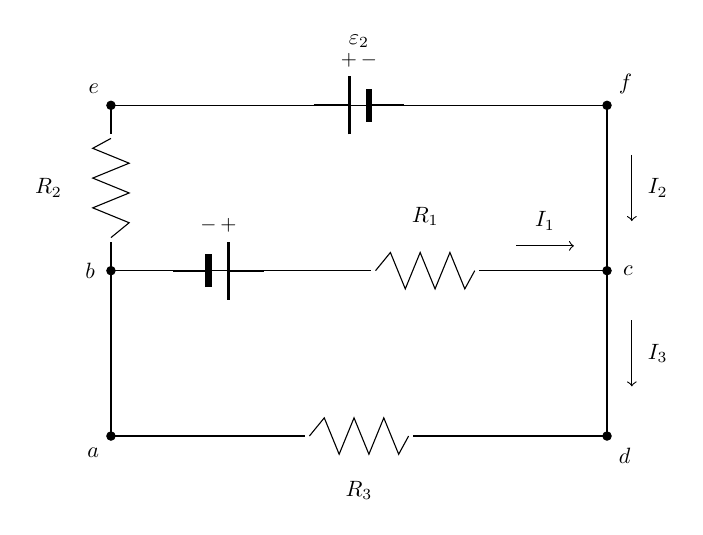
\begin{tikzpicture}[x=1.05cm,y=1.05cm]
  \draw (0,0) -- (0,4) (6,0) -- (6,4) (0,4) -- (6,4) (0,0) -- (6,0) (0,2) -- (6,2);
  \batthL{3,4}
  \node[scale=0.8, anchor=south] at (3,4.6) {$\varepsilon_2$};
  \reszigv{0,3}
  \node[scale=0.8, anchor=east] at (-0.5,3) {$R_2$};
  \batthR{1.3,2}
  \reszig{3.8,2}
  \node[scale=0.8, anchor=south] at (3.8,2.45) {$R_1$};
  \draw[->] (4.9,2.3) -- (5.6,2.3);
  \node[scale=0.8] at (5.25,2.6) {$I_1$};
  \draw[->] (6.3,3.4) -- (6.3,2.6);
  \node[scale=0.8, anchor=west] at (6.4,3) {$I_2$};
  \draw[->] (6.3,1.4) -- (6.3,0.6);
  \node[scale=0.8, anchor=west] at (6.4,1) {$I_3$};
  \reszig{3,0}
  \node[scale=0.8, anchor=north] at (3,-0.45) {$R_3$};
  \twoloopdots
\end{tikzpicture}
\end{center}

Write the loop rule for each loop and the junction rule at $c$, then solve
the resulting system for all three currents.

\derivbox{4.2cm}{Loop 1 (through $\varepsilon_2,R_2$):
$I_1R_1-I_2R_2=\varepsilon_1+\varepsilon_2$ \par Loop 2 (through $R_3$):
$I_1R_1+I_3R_3=\varepsilon_1$ \par Junction at $c$: $I_1+I_2=I_3$}

\eqline[0.1cm]{$I_1 = $}
\eqline[0.1cm]{$I_2 = $}
\eqline[0.1cm]{$I_3 = $}

\checkpoint{One of your currents came out negative. What does that tell you
about the direction you assumed for it on the diagram?}

%============================================================
\nsec{Problem 5 --- an unknown resistor}

Same shape, new numbers: $\varepsilon_1=20$ V, $R_1=3\ \Omega$,
$\varepsilon_2=10$ V, $R_2=5\ \Omega$. This time $R_3$ is unknown --- but an
ammeter in the $\varepsilon_1$-$R_1$ branch reads $I_1=4.0$ A.

\begin{center}
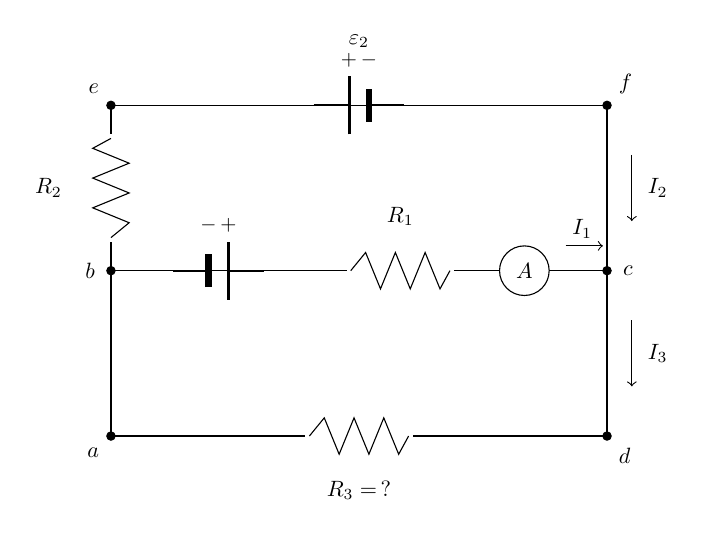
\begin{tikzpicture}[x=1.05cm,y=1.05cm]
  \draw (0,0) -- (0,4) (6,0) -- (6,4) (0,4) -- (6,4) (0,0) -- (6,0) (0,2) -- (6,2);
  \batthL{3,4}
  \node[scale=0.8, anchor=south] at (3,4.6) {$\varepsilon_2$};
  \reszigv{0,3}
  \node[scale=0.8, anchor=east] at (-0.5,3) {$R_2$};
  \batthR{1.3,2}
  \reszig{3.5,2}
  \node[scale=0.8, anchor=south] at (3.5,2.45) {$R_1$};
  \metercirc{5,2}{A}
  \draw[->] (5.5,2.3) -- (5.95,2.3);
  \node[scale=0.8, anchor=south] at (5.7,2.3) {$I_1$};
  \draw[->] (6.3,3.4) -- (6.3,2.6);
  \node[scale=0.8, anchor=west] at (6.4,3) {$I_2$};
  \draw[->] (6.3,1.4) -- (6.3,0.6);
  \node[scale=0.8, anchor=west] at (6.4,1) {$I_3$};
  \reszig{3,0}
  \node[scale=0.8, anchor=north] at (3,-0.45) {$R_3=\,?$};
  \twoloopdots
\end{tikzpicture}
\end{center}

Use the loop rule and the junction rule to find $R_3$. (Work out $I_2$,
then $I_3$, on your way there.)

\derivbox{4.2cm}{Loop 1 gives $I_2$; the junction rule gives $I_3$; Loop 2
($\varepsilon_1=I_1R_1+I_3R_3$) then gives $R_3$}

\eqline[0.1cm]{$I_2 = $}
\eqline[0.1cm]{$I_3 = $}

\result[1cm]{$R_3 = $}

\checkpoint{Could you have found $R_3$ without first finding $I_2$? Why or
why not?}

%============================================================
\nsec{Problem 6 --- an unknown EMF}

Same shape again: $R_1=5\ \Omega$, $R_2=6\ \Omega$, $R_3=4\ \Omega$. This
time $\varepsilon_2$ is unknown, but $\varepsilon_1=21$ V is given, and the
ammeter reads $I_1=3.0$ A.

\begin{center}
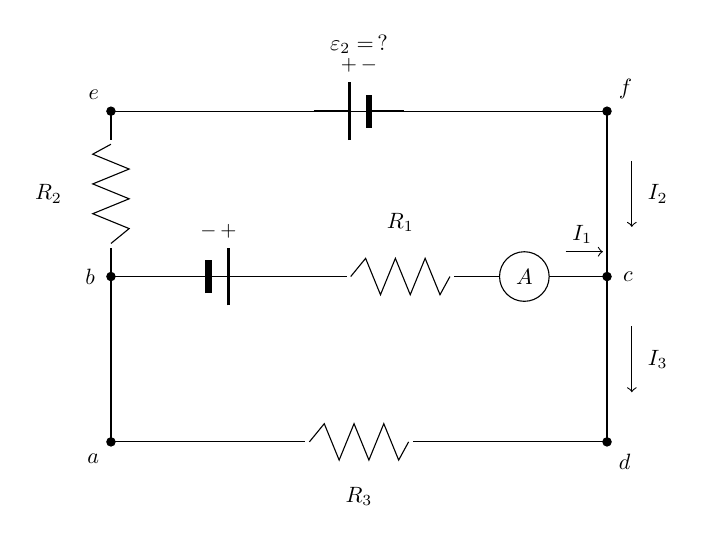
\begin{tikzpicture}[x=1.05cm,y=1.05cm]
  \draw (0,0) -- (0,4) (6,0) -- (6,4) (0,4) -- (6,4) (0,0) -- (6,0) (0,2) -- (6,2);
  \batthL{3,4}
  \node[scale=0.8, anchor=south] at (3,4.6) {$\varepsilon_2=\,?$};
  \reszigv{0,3}
  \node[scale=0.8, anchor=east] at (-0.5,3) {$R_2$};
  \batthR{1.3,2}
  \reszig{3.5,2}
  \node[scale=0.8, anchor=south] at (3.5,2.45) {$R_1$};
  \metercirc{5,2}{A}
  \draw[->] (5.5,2.3) -- (5.95,2.3);
  \node[scale=0.8, anchor=south] at (5.7,2.3) {$I_1$};
  \draw[->] (6.3,3.4) -- (6.3,2.6);
  \node[scale=0.8, anchor=west] at (6.4,3) {$I_2$};
  \draw[->] (6.3,1.4) -- (6.3,0.6);
  \node[scale=0.8, anchor=west] at (6.4,1) {$I_3$};
  \reszig{3,0}
  \node[scale=0.8, anchor=north] at (3,-0.45) {$R_3$};
  \twoloopdots
\end{tikzpicture}
\end{center}

Find $\varepsilon_2$. (This time work out $I_3$ first, then $I_2$.)

\derivbox{4.2cm}{Loop 2 ($\varepsilon_1=I_1R_1+I_3R_3$) gives $I_3$; the
junction rule gives $I_2$; Loop 1 then gives $\varepsilon_2$}

\eqline[0.1cm]{$I_3 = $}
\eqline[0.1cm]{$I_2 = $}

\result[1cm]{$\varepsilon_2 = $}

\checkpoint{Compare the order you worked in for Problems 5 and 6 --- which
loop did you need \emph{first} in each, and why did the unknown force that
order?}

\end{document}
